\documentclass[12pt,a4paper,oneside]{report}

% Page layout
\usepackage[a4paper,top=1.7cm,bottom=7.4cm,left=2.5cm,right=6.0cm,footskip=6.3cm]{geometry}
\usepackage{setspace}
\usepackage{titlesec}
\usepackage{titling}
\usepackage{times}
\usepackage{fontspec}
\setmainfont{Arial}
\usepackage{fancyhdr}
\pagestyle{fancy}
\fancyhf{}
\fancyfoot[C]{\thepage}
\renewcommand{\headrulewidth}{0pt}
\renewcommand{\footrulewidth}{0pt}

% Include PDF
\usepackage{pdfpages}
% Bibliography
\usepackage{natbib}
\bibliographystyle{plain}  % or another style that suits your needs
\usepackage{url}
\usepackage{hyperref}

% Paragraph formatting
\setlength{\parskip}{6pt}
\setlength{\parindent}{0pt}
\setstretch{1.5}

\begin{document}

% Include the first page from the PDF file
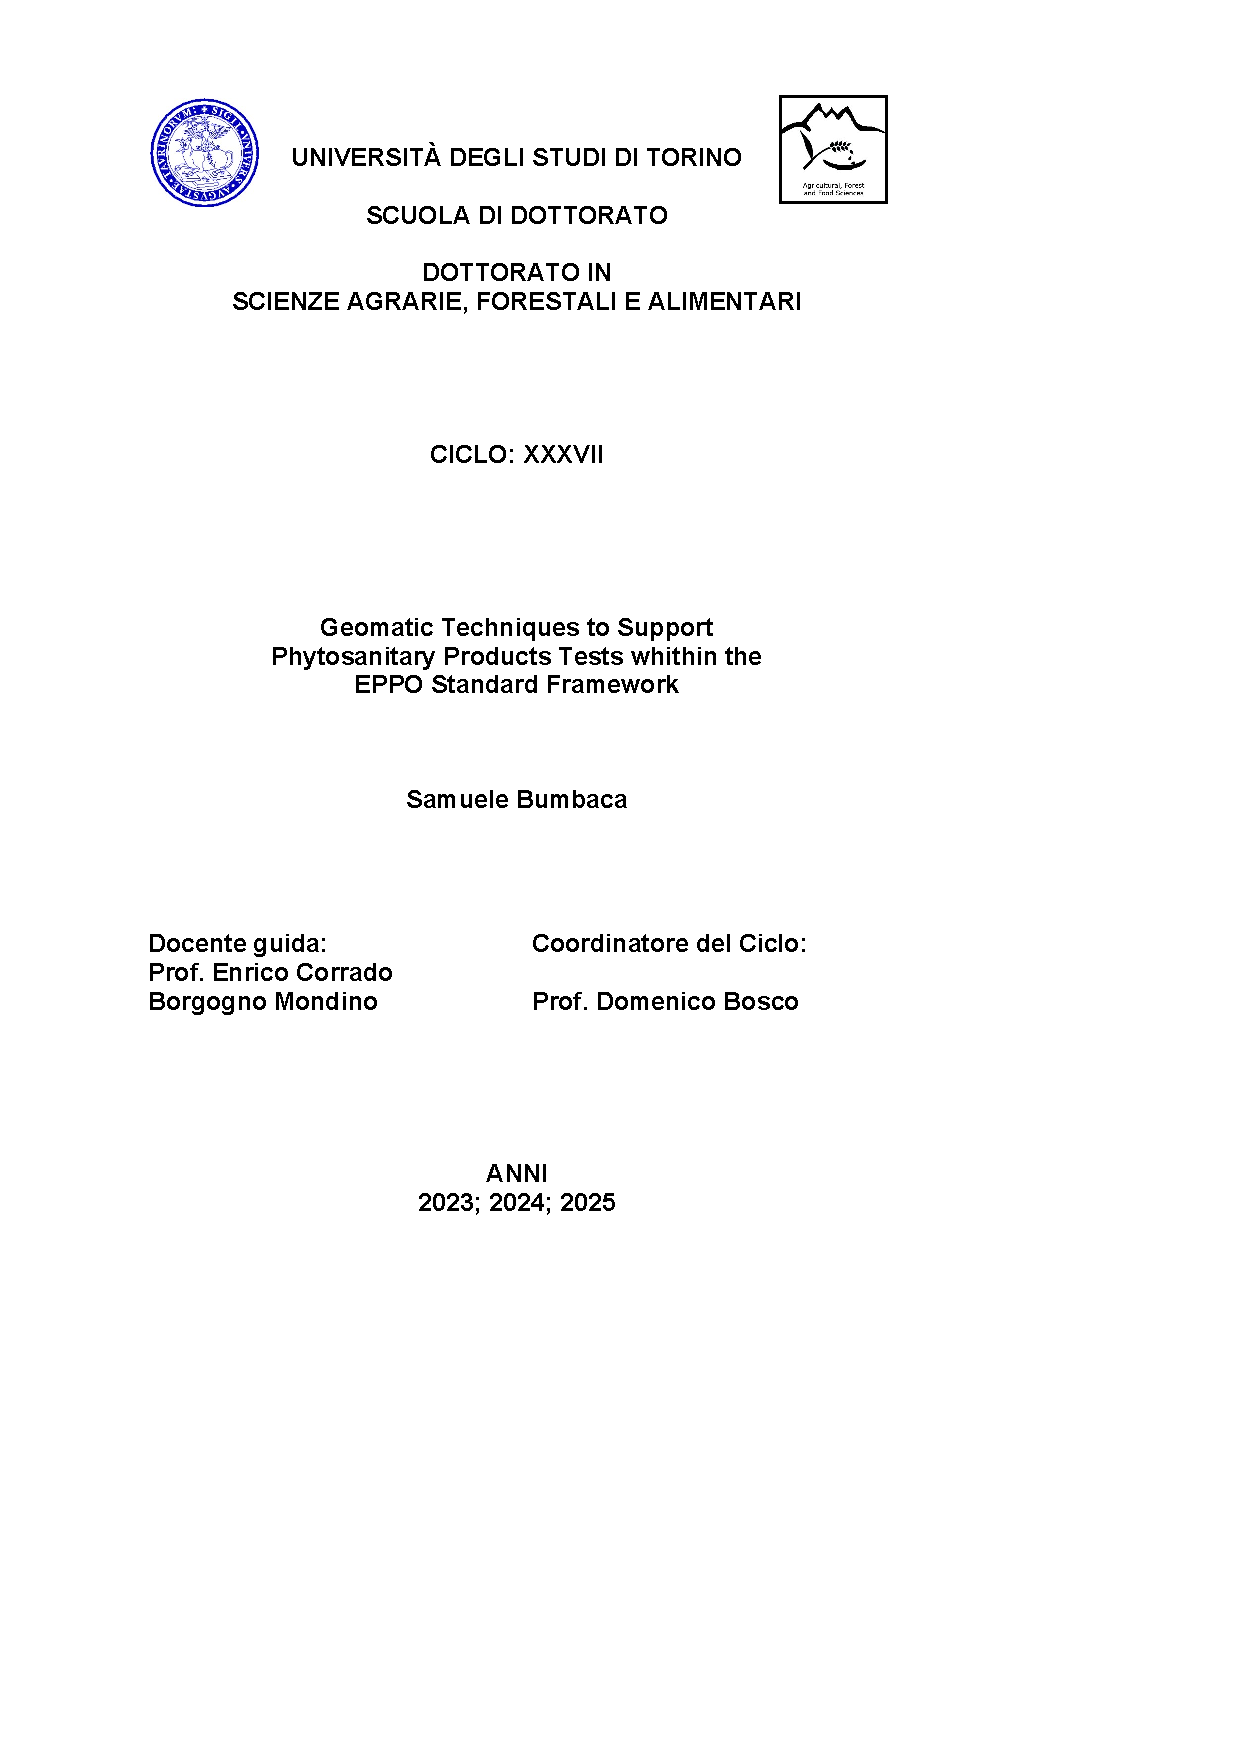
\includepdf[pages=1]{Intestazione/t3._Thesis_first_page.pdf}

% Table of Contents
\tableofcontents
\newpage

% Main content
\chapter{Introduction}

\section{EPPO}
\subsection{Phytosanitary Products}

Phytosanitary products, commonly used as a synonym for "Plant Protection Products" (PPPs),
are a specific category of pesticides designed primarily to maintain crop health 
and prevent destruction by diseases and infestations. While the term "pesticides" 
is broader and also includes biocidal products used to control harmful organisms 
and disease carriers not related to plant protection, phytosanitary products are 
specifically used to control harmful organisms affecting cultivated plants (such 
as insects, mites, fungi, bacteria, rodents, etc.), eliminate weeds, and regulate 
plant physiological processes. Fertilizers, which serve for plant nutrition and 
soil fertility improvement, are excluded from phytosanitary products.

Phytosanitary products contain at least one active substance, which can be either 
chemical compounds or microorganisms, including viruses, that enable the product 
to perform its intended function. These active substances undergo rigorous risk 
assessment processes, with EFSA (European Food Safety Authority) playing a central 
role in conducting peer reviews at the EU level to determine if these products, 
when used correctly, might produce harmful effects on human or animal health, either 
directly or indirectly through drinking water, food, or feed.

The main categories of phytosanitary products can be distinguished based on the 
type of organism they target or the function they perform, including:


\begin{itemize}
    \item Fungicides
    \item Insecticides
    \item Acaricides
    \item Rodenticides
    \item Slimicides
    \item Nematicides
    \item Herbicides
    \item Plant growth regulators
\end{itemize}

The parameters identified through the risk assessment are compared with the values 
established by directive 97/57/EC \cite{EURLex1997265}, which indicates the acceptability limits for 
decision-making on the inclusion of active substances in the EU list (Annex I of 
directive 91/414/EEC \cite{directive_91_414_EEC}).

The Introduction of a product in the EU market is not only subject to audits on
active substances and their safety for humans and environment but also to the evaluation 
of the product's efficacy and safety for the crop.
World Trade Organization Sanitary and Phytosanitary Measures Agreement \cite{WTO_SPS_Agreement}
recognizes the International Plant Protection Convention (IPPC) as the only international
institution in charge of emitting standards for plant health \cite{IPPC}. IPPC is organized in
regions. European Union (EU) countries refer to the European and Mediterranean Plant
Protection Organization (EPPO). EPPO Standards are divided into Standards on
Phytosanitary Measures and Standards on PPPs. PPPs standards describe the efficacy
evaluation of PPPs (PP 1) and good plant protection practices. EU GEP units provide
Biological Assessment Dossier (BAD) efficacy trials. GEP units are expected to follow
EPPO PP 1 to assess PPPs selectivity detecting phytotoxicity effects, and efficacy in the
complaint of Regulation (EC) No 1107/2009 of the European Parliament and Council \cite{EC_Regulation_1107_2009}.

\subsection{Standard Experimental Design}

Generics on efficacy assessments are reported in PP 1/181(5) \cite{EPPO_PP1_181}, which describes
herbicide, fungicide, bactericide, and insecticide efficacy on the target evaluation.
PP 1/135(4) \cite{EPPO_PP1_135} describes the selectivity assessment procedures, 
in other words: the standard phytotoxicity assessments of PPPs.
The PP 1/152 \cite{EPPO_PP1_152} standard describes the general principles for the
efficacy and selectivity evaluation of PPPs, in describing the standard experimental design.
Aside from: objectives of the study, description of treatments, controls, reference treatment, 
plot size, replications, randomization, sampling and assessment timing, the
PP 1/152 outlined that a comprehensive experimental design should include:
a description of the sampling and measurement procedures and the statistical analysis plan.

Target and crop-specific standards point out "mode of
assessment recording and measurements" fixing evaluation metrics in two ways:
countable (discrete values) and measurable (continuous values) effects which must be
expressed in absolute values, in other cases, frequency (incidence) and degree
(severity) should be estimated and reported as affected percentage of the individual (ex.
plant or plot) or as proportion within thesis and control expressed in percentage. As
specified by PP 1/152 \cite{EPPO_PP1_152}, classification by ranking (ordinal) and scoring (ordinal or
nominal) is also contemplated. In the case of estimation, rather than count or measure,
PP 1/152 reports "The observer should be trained to make the estimations and his
observations should be calibrated against a standard". Calibration compliance with
standards is ensured by GEP audits. Scoring and ranking scales examples are
published on specific standards or the same PP 1/152. The lack of specific scales lets
trial protocol authors define one inspired in range and intervals by the mentioned
examples or other well-established ones.
GEP units PP 1 assessments are produced by trained and experienced
agronomists or biologists by visual inspection or laboratory analysis. The technician
follows the trial protocol and related EPPO standards during assessment execution. The
technician is critical for accuracy, precision, and repeatability. Sensitivity is determined
by the trial protocol. It depends on expected differences and if a measure, a proportion,
or a scale is used. For instance, in PP 1/93(3) \cite{EPPO_PP1_93} "Efficacy evaluation of herbicides -
Weeds in cereals - Observation on the crop", phytotoxicity color modification could be
measured, or estimated as proportion in respect to the untreated, or scored in EPPO
scale as PP 1/135(4) reports, or a scientifically accepted score as the European Weed
Research Society phytotoxicity damage score \cite{EWRS_score} and other ones.
In general, data types must undergo the classification presented in Table 1.1

\begin{table}[ht]
\caption{Different modes of observation and types of variables}
\label{tab:data_types}
\centering
\begin{tabular}{|l|c|c|c|c|}
\hline
\textbf{Type of Variable} & \textbf{Measurement} & \textbf{Visual Estimation} & \textbf{Ranking} & \textbf{Scoring} \\
\hline
Binary & & & & X \\
\hline
Nominal & & & & X \\
\hline
Ordinal & & & X & X \\
\hline
Discrete & X & X & & \\
\hline
Continuous limited & X & X & & \\
\hline
Continuous not limited & X & X & & \\
\hline
\end{tabular}
\end{table}

The statistical analysis of trials is equally critical, providing objective 
assessment of treatment effects. While PP 1/152 \cite{EPPO_PP1_152} doesn't prescribe 
specific analyses for all situations, it emphasizes that analysis methods should 
align with the experimental design and data types collected. For qunatitative 
variables (continuous or discrete), parametric methods based on Generalized 
Linear Models (GLM) are recommended, including ANOVA and regression approaches. 
For qualitative variables (ordinal or nominal), non-parametric methods are more 
appropriate. Parametric analysis assumes additivity of effects, homogeneity of variance, 
and normally distributed errors—when these assumptions aren't met, data transformations 
or alternative approaches become necessary.

Statistical tests, particularly F-tests of orthogonal 
contrasts, should focus on biologically relevant comparisons specified during the 
design stage: untreated control versus treatments (establishing trial validity), 
reference products versus control (demonstrating coherence), test products versus 
reference (evaluating efficacy), and comparisons among test products (identifying 
superior treatments). For efficacy trials, EPPO suggests one-sided tests since the 
aim is comparing products against references or controls, with appropriate multiple 
comparison procedures when needed.

Through adherence to these rigorous design and analysis standards, researchers can 
generate reliable evidence to support phytosanitary product registration while ensuring 
that products demonstrate consistent efficacy across relevant agricultural conditions.

\subsection{Digital Approaches}

While the EPPO experimental design standards provide a solid foundation for conducting
phytosanitary product trials, the increasing availability of digital tools and technologies
offers new opportunities to enhance the efficiency and accuracy of these assessments.
Digital approaches can streamline data collection, automate analysis, and improve the
reproducibility of results, ultimately accelerating the development and registration of
effective phytosanitary products.

In November 2024, the EPPO published a new standard, PP 1/333(1) \cite{PP13332024}, which 
filled the gap in the use of digital technologies in phytosanitary product efficacy
and selectivity trials. This standard provides guidelines for incorporating digital
tools into trial protocols, including the use of digital sensors and algorithms
for data processing and analysis.

When implementing digital technologies in efficacy trials, it is essential to document how the technology was used in accordance with the verification report. In the final trial report, digital technologies used in assessment should be clearly specified, including:

- The type of digital technology used and its version number
- Reference to the verification report
- Confirmation that the digital technology was used within its verified scope and operating conditions
- Any deviations from the standard operating procedure and their potential impact on the results
- Calibration records showing the equipment was operating correctly at the time of assessment

The data generated through digital technologies should be stored in a manner that ensures traceability and allows for subsequent verification if required by regulatory authorities. Raw data, such as images used for analysis, should be archived according to GEP requirements.


Digital technologies offer significant potential to enhance the accuracy, efficiency, and reproducibility of efficacy evaluations for plant protection products. When properly validated, verified, and calibrated, these technologies can complement or potentially replace conventional assessment methods while maintaining compliance with GEP standards.

As digital technologies continue to evolve, this Standard will be periodically reviewed and updated to reflect advancements in hardware capabilities, algorithm development, and machine learning applications. Regulatory authorities, GEP facilities, and technology developers are encouraged to collaborate in the ongoing development of appropriate standards for digital technology implementation in efficacy evaluation trials.

The adoption of digital technology should prioritize data quality, reliability, and transparency while facilitating innovation that may improve the assessment of plant protection product performance. All parties involved should work to ensure that digital technologies are implemented in a manner that maintains the scientific integrity of efficacy evaluations while enabling more efficient and potentially more precise data collection methodologies.

\section{Geomatic Technics}
\subsection{Photogrammetry}
\subsection{Geostatistics}

\section{Machine Learning}
\subsection{Approaches}
\subsection{Computer Vision}


\chapter{Thesis Aims and Framework: A New Statistical Analysis Workflow}

\chapter{Study Cases}
\section{Continuous Variables}
\subsection{Plant Count}

\section{Ordinal and Nominal Variables}
\subsection{Phytoxicity Score}

\section{Binary Variables}
\subsection{Embedding Spaces for Control Sample Anomaly Detection}

\bibliographystyle{plainnat}
\bibliography{Phd_Thesis_SBumbaca}

\end{document}